\section{Aufbau und Durchführung}
\label{sec:Aufbau}
\subsection{Aufbau}
Der verwendete Versuchsaufbau ist in \autofref{pic:Aufbau_Foto} zu sehen. Grundlegend für den Versuch ist der Rezipient, der die Probe in einem Vakuum hält. Als Probe wird mit Strontium dotiertes Kaliumbromid verwendet. Diese ist innerhalb des Rezipient auf den Boden aufgekittet, wie in \autoref{pic:Rezipient_Foto} zu sehen. Auf der Probe ist eine Metallplatte angebracht, sodass zwischen Boden und Metallplatte eine Spannung mithilfe des Spannungsgenerators angelegt werden kann. Der Boden des Rezipienten ist außerdem mit dem Kühlfinger verbunden, der in ein Dewar Gefäß reicht, welches mit flüßigem Stickstoff gefüllt werden kann. Das Dewargefäß steht auf einem höhenverstellbaren Tisch. Am Rezipienten 
\begin{figure}
    \centering
    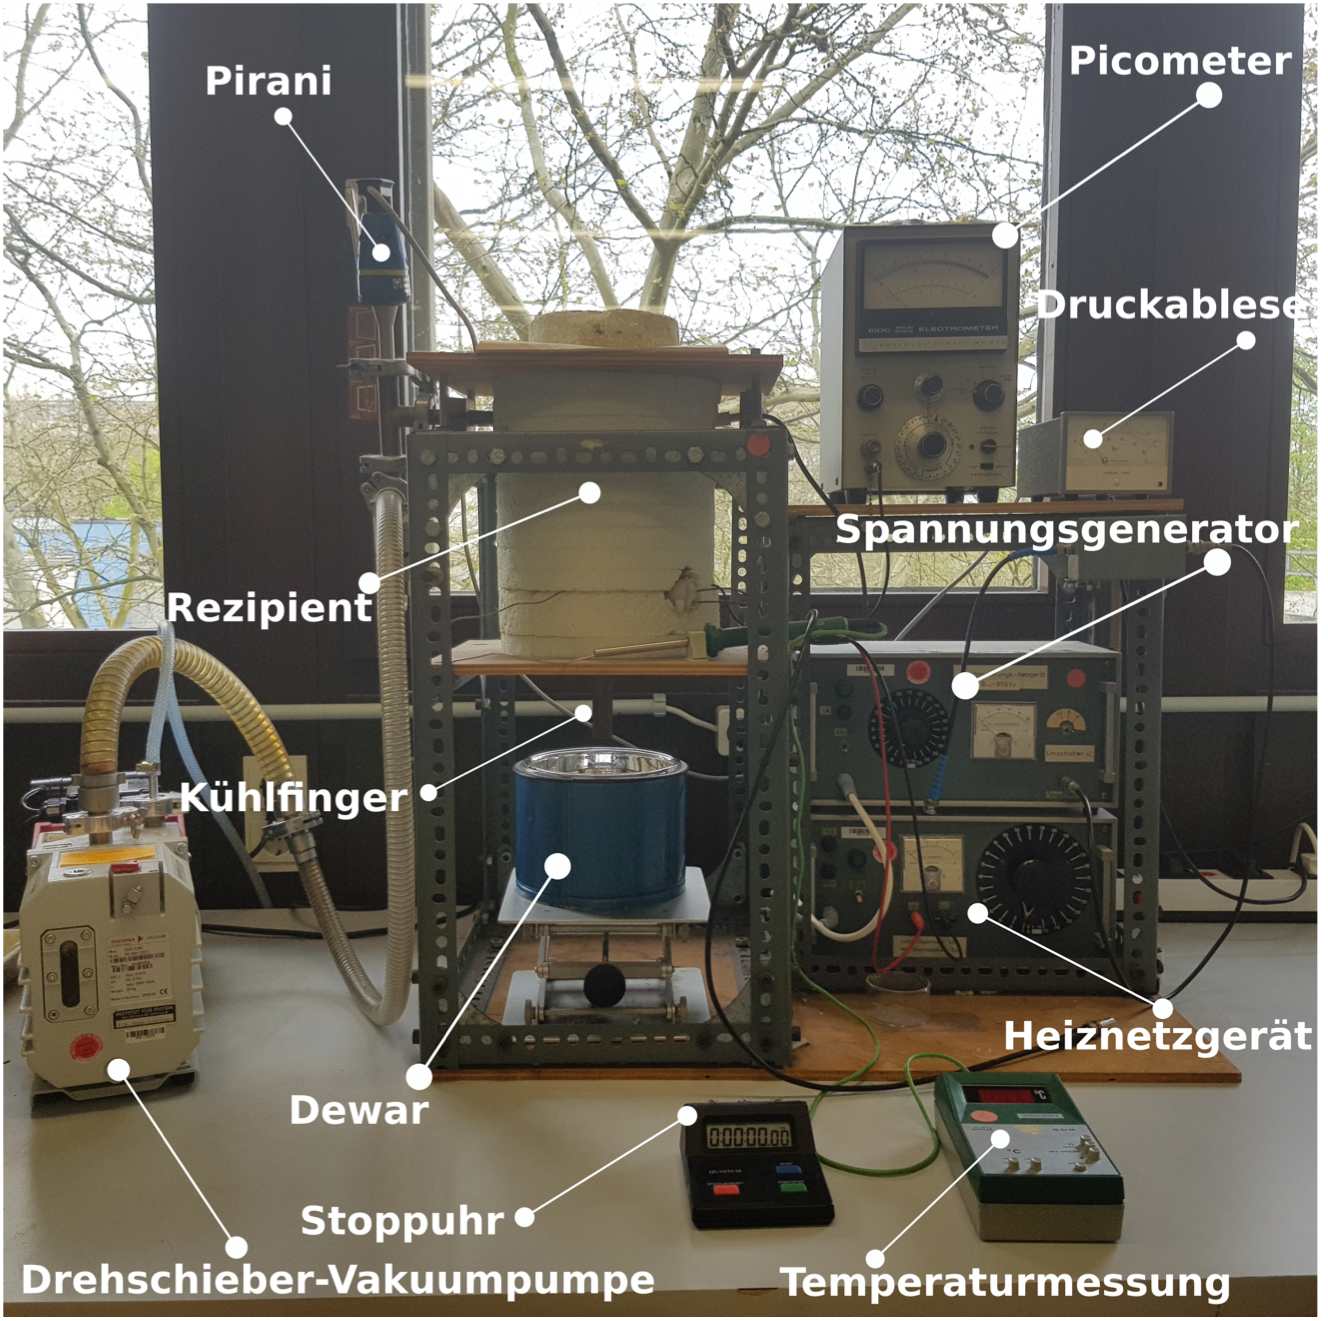
\includegraphics[width=0.5\linewidth]{Bilder/Aufbau.jpeg}
    \caption{Foto des Versuchsaufbaus mit Beschriftung der Bestandteile.\cite{anleitungV48}}
    \label{pic:Aufbau_Foto}
\end{figure}
\begin{figure}
    \centering
    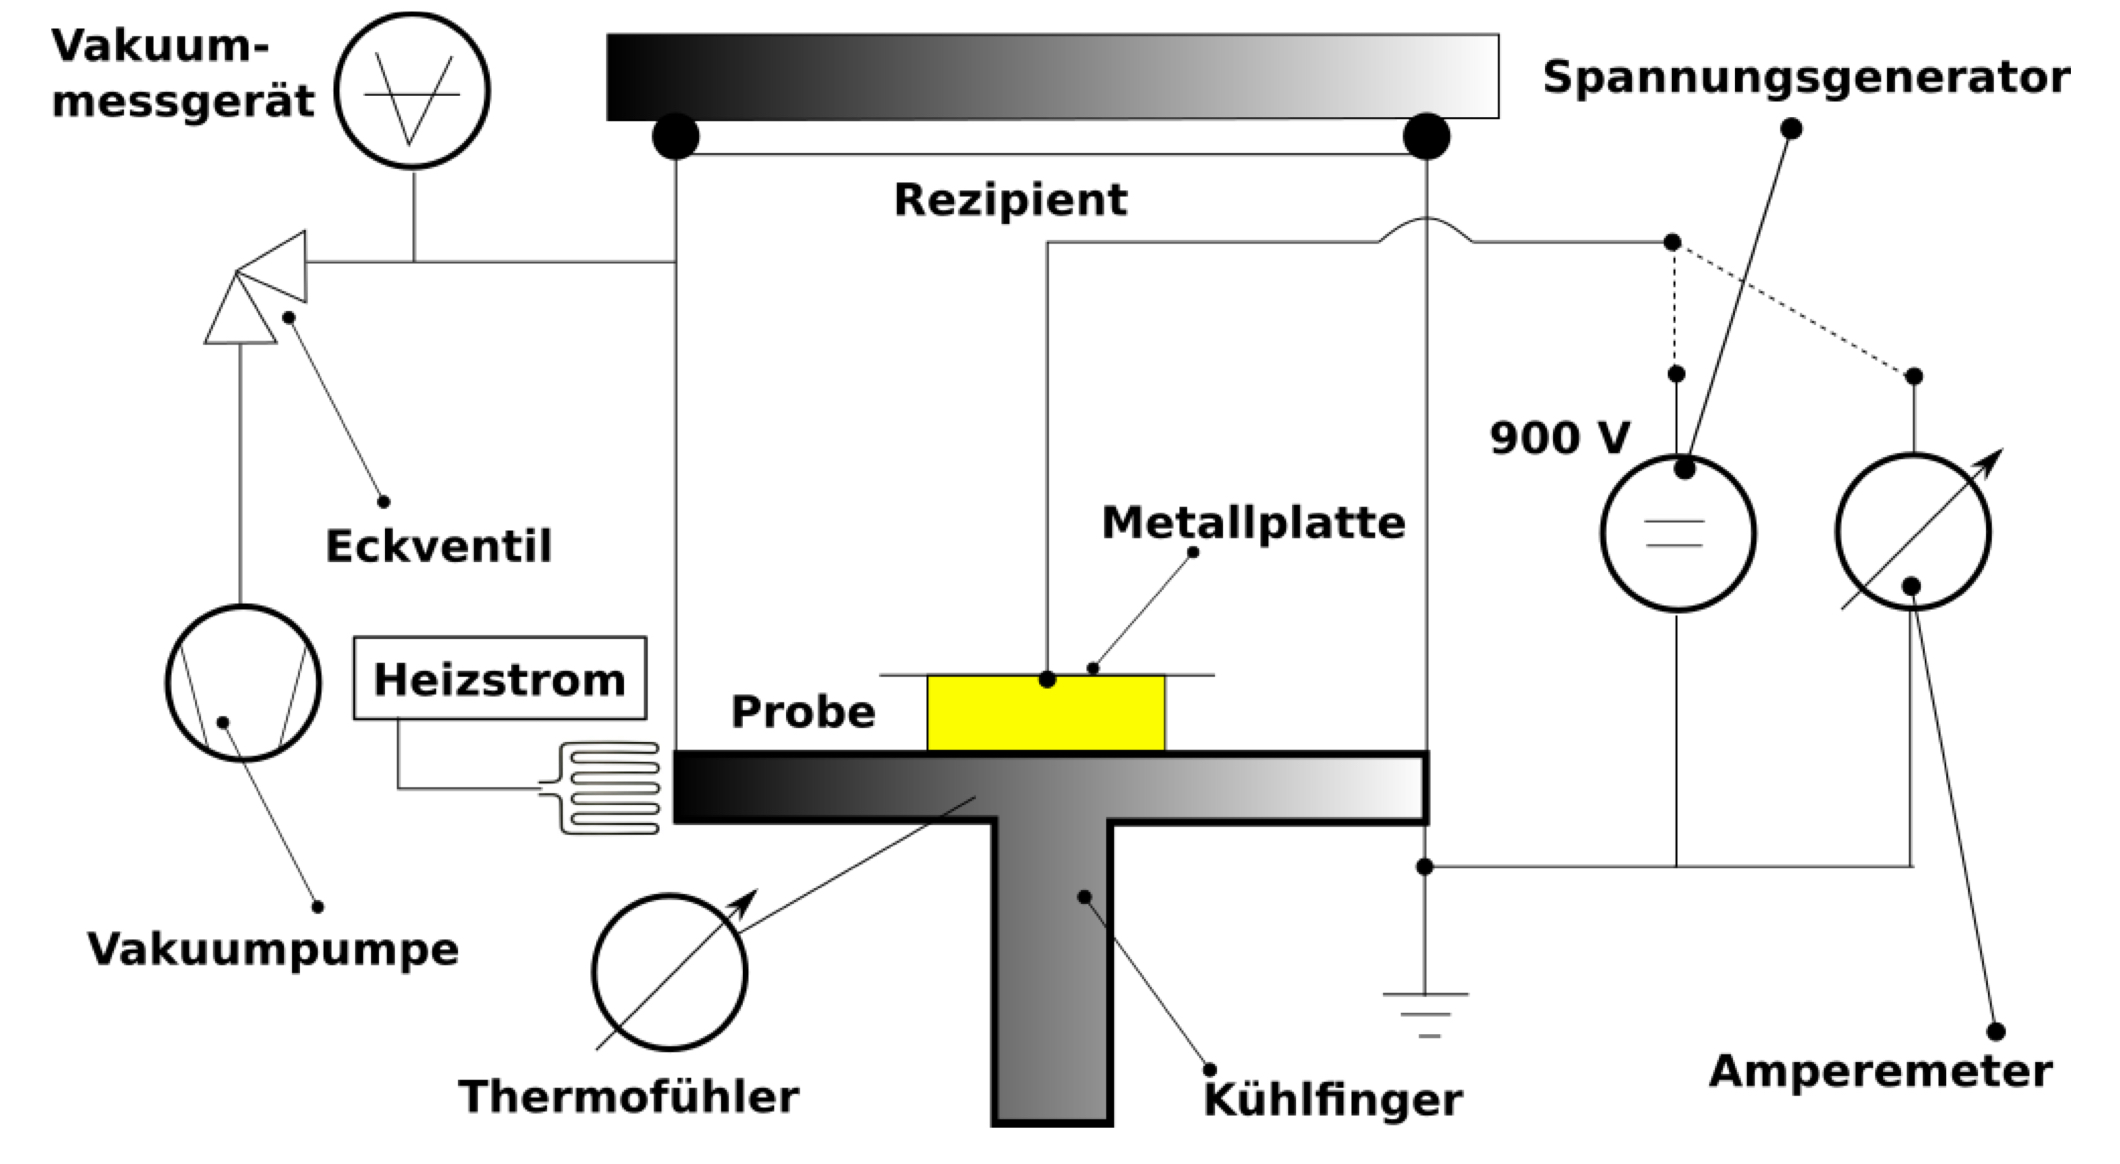
\includegraphics[width=0.5\linewidth]{Bilder/Rezipient.jpeg}
    \caption{Schematische Darstellung des Rezipienten und anliegender Messtechnik.\cite{anleitungV48}}
    \label{pic:Rezipient_Foto}
\end{figure}
\subsection{Durchführung}
\label{sec:Aufbau}